\section{Elbow Curve}
Elbow Curve (dirsek eğrisi), kümeleme algoritmalarında optimal küme sayısını belirlemek için kullanılan bir tekniktir. Her bir küme sayısı için kümeleme performansını ölçer ve küme sayısının artmasıyla birlikte kümeleme performansındaki iyileşmeyi gösterir. Küme sayısını artırmak kümeleme performansında belirgin bir iyileştirme sağlamazsa bu nokta optimal küme sayısı olarak kabul edilir.

\begin{lstlisting}[language=Python]
import numpy as np
import matplotlib.pyplot as plt
from sklearn.cluster import KMeans
from sklearn.datasets import make_blobs

# Ornek veri seti olusturma
X, _ = make_blobs(n_samples=300, centers=4, cluster_std=0.60, random_state=0)

# Kume sayisi araligi belirleme
k_range = range(1, 11)

# SSE degerlerini depolamak icin bos bir liste olusturma
sse = []

# Farkli kume sayilari icin KMeans modeli olusturma ve SSE degerlerini hesaplama
for k in k_range:
    kmeans = KMeans(n_clusters=k)
    kmeans.fit(X)
    sse.append(kmeans.inertia_)

# Elbow curve grafigi olusturma
plt.plot(k_range, sse, marker='o')
plt.show()
\end{lstlisting}

\begin{figure}[h]
    \centering
    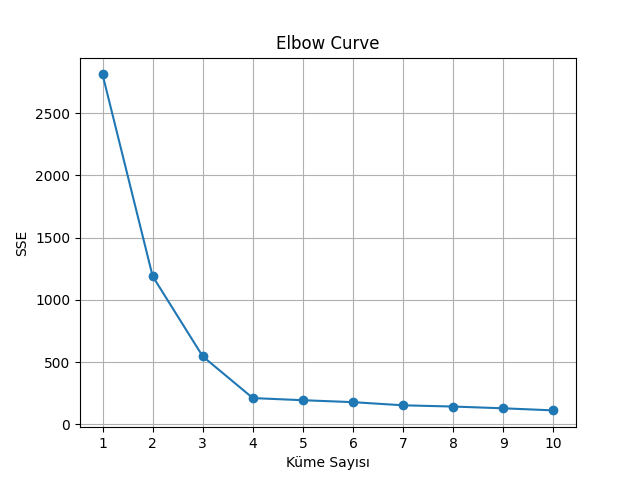
\includegraphics[width=0.4\textwidth]{images/elbow_curve.png}
    \caption{Elbow Curve örneği.}
    \label{fig:enter-label}
\end{figure}

\newpage